\documentclass{article}
\usepackage{a4wide}
\usepackage{graphicx}
\usepackage{amsmath, amsthm, amssymb}

\usepackage[utf8]{inputenc}
\usepackage{ngerman}
\usepackage{url}
\usepackage[ruled,vlined]{algorithm2e}
\usepackage[]{hyperref}
\usepackage{listings}
\usepackage{dsfont}

\newtheorem{thm}{Theorem}[section]
\newtheorem{cor}[thm]{Korollar}
\newtheorem{lem}[thm]{Lemma}
\newtheorem{defi}[thm]{Definition}
\newtheorem{definition}{Definition}
\newcounter{Chapcounter}
\newcommand\showmycounter{\addtocounter{Chapcounter}{1}\themycounter}
\newcommand{\chapter}[1] 
{ {\centering          
  \addtocounter{Chapcounter}{1} \Large \underline{\textbf{ \color{blue} Chapter \theChapcounter: ~#1}} }   
  \addcontentsline{toc}{section}{ \color{blue} Chapter:~\theChapcounter~~ #1}    
}
\hypersetup{colorlinks=true}
\hypersetup{linkcolor=black}
\usepackage{listings}
\lstdefinelanguage{Pseudo}{
  morekeywords={forall,if,then,else,return,while,do,for,DFS},
  sensitive=false,
  morecomment=[l]{//},
  morestring=[b]"
}



\setcounter{tocdepth}{4}

\begin{document}
\title{Modellierung}
\date{Sommersemester 2026}
\author{Universität Stuttgart}
\maketitle
\tableofcontents
\newpage

\section{Preface}
This lecture is in english so I hope all vocabulary will be adecuately written in engish.

These notes contain all topics I valued as important for the exam, but some stuff that may have been trivial for me may not appear in the notes. So if anybody is using my notes to 
prepare for the exam, please be wary of this.

UPDATE: Given the official notes are already in english, I will partially be abandoning the development of these notes. Should \textbf{not} be used to rely on studying for the exam.
\section{Alias List}
\begin{itemize}
  \item OLTP (On-Line Transaction Processing)
  \item DW (Data Warehouse)
  \item OLAP (On-Line Analytical Processing): analysis of business data
  \item ROLAP (Relational OLAP)
  \item MOLAP (Multidimensional OLAP)
  \item DSS (Decision Support System)
  \item KDD (Knowledge Discovery in Databases), often used as a synonym for Data Mining
\end{itemize}

\section{Course Overview / Organization}
This course is based on two main parts:
\begin{itemize}
  \item Databases and the languages used to interact with them
  \item System and process models (e.g., XML, UML)
\end{itemize}

\textbf{Exam (Schein):} 60 minutes, closed book.  
To qualify, you need to pass both the exercises and the mock exam.

\section{Database Management System (DBMS)}
A DBMS is a system for managing \textbf{large} amounts of data, enabling efficient, concurrent, and secure access.

\subsection{Core Aspects}
\begin{itemize}
  \item Modeling and design of the database
  \item Queries and database operations (programming)
  \item DBMS implementation
\end{itemize}

\subsection{Data Models}
Data models describe entities and their relationships.

Example: A \textbf{student} enrolls in a \textbf{course} given by a \textbf{lecturer}.

\subsubsection{Constructors}
Constructors define data structures and their operations.

\begin{lstlisting}
CREATE TABLE STUDENT (
  MATRIKELNUMBER INTEGER,
  LASTNAME VARCHAR(40),
  FIRSTNAME VARCHAR(40),
  BIRTHDATE CHAR(8),
  ...
);
\end{lstlisting}

\subsubsection{Notion of Model}
A model is a set of language features used to describe a universe of discourse.

\textit{(Note: 'universe of discourse' = the domain of interest being modeled.)}

\subsection{Databases}
The goal is to separate data from applications, so data can be reused independently of implementation details.

This also enables flexibility for integrating new applications.

\subsubsection{Transactions (ACID)}
\begin{itemize}
  \item \textbf{Atomicity}: Either all changes happen or none
  \item \textbf{Consistency}: Data remains valid after a transaction
  \item \textbf{Isolation}: Transactions do not interfere with each other
  \item \textbf{Durability}: Changes persist even after failures
\end{itemize}

\subsubsection{Fault Tolerance}
Achieved through logging and recovery mechanisms.

\subsubsection{Multi-user Operation}
Supports concurrent access by multiple users.

\section{Computer-Based Information Systems (CIS)}
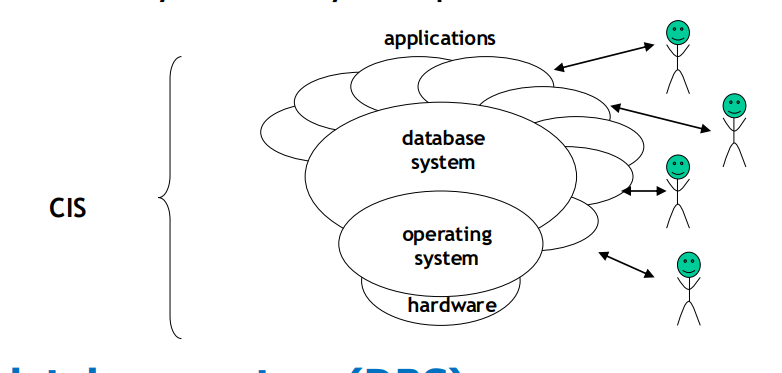
\includegraphics[scale=0.5]{assets/cis.png}

\subsection{Database System (DBS)}
A database system consists of:
\begin{itemize}
  \item A \textbf{database}
  \item A \textbf{DBMS}
\end{itemize}

\subsubsection{Classical Data Models}
\begin{itemize}
  \item Relational model (tables)
  \item Network model (graph-based)
  \item Hierarchical model (tree structure)
\end{itemize}

Typically, these use fixed record structures.

\subsubsection{DBS Interface}
\begin{itemize}
  \item Define object types
  \item Query and update data
  \item Define constraints
  \item Manage access control (permissions)
\end{itemize}

\subsection{Business Information Systems}
Requirements are divided into three levels:
\begin{itemize}
  \item Operational level (e.g., clerks)
  \item Middle management level
  \item Strategic level (e.g., board of directors)
\end{itemize}

\section{Web-Based Application Architecture}
Based on internet technologies (e.g., TCP/IP, HTTP).

\section{Data Warehouse (DW)}
Allows efficient access to aggregated data (e.g., total sales per quarter) without scanning the entire database.

Used for very large datasets (e.g., TiB scale) via incremental aggregation.

\subsection{Data Mining}
Data mining is the process of discovering hidden, previously unknown, and useful information from large datasets.

It is typically exploratory (no predefined expectations) and helps improve understanding of the data.

\section{Data Abstraction}
\begin{itemize}
  \item \textbf{View level}: User-specific view, simplified and application-dependent
  \item \textbf{Logical level}: Used by database administrators, more detailed structure
  \item \textbf{Physical level}: Describes how data is actually stored
\end{itemize}

\subsection{Three-Schema Architecture}
\begin{itemize}
  \item \textbf{Conceptual schema} (logical view): Overall structure of the database (uses DDL)
  \item \textbf{External schema} (user view): Specific parts relevant to users
  \item \textbf{Internal schema}: Physical storage and access paths
\end{itemize}

\section{Database design}
Model of a part of the real world. That information is stored as data.

It should be simple, understandable and easy to read.

\section{Entity-Relationship Model}

\subsection{Keys}
\begin{itemize}
  \item Super key: Set of one or more attributes that uniquely determine an entity
  \item Candidate key: Minimal super key
  \item Primary Key: One of the candidate keys that is set as 'the key' of the entity set.
\end{itemize}

Weak entity set: Entity set without a primary key

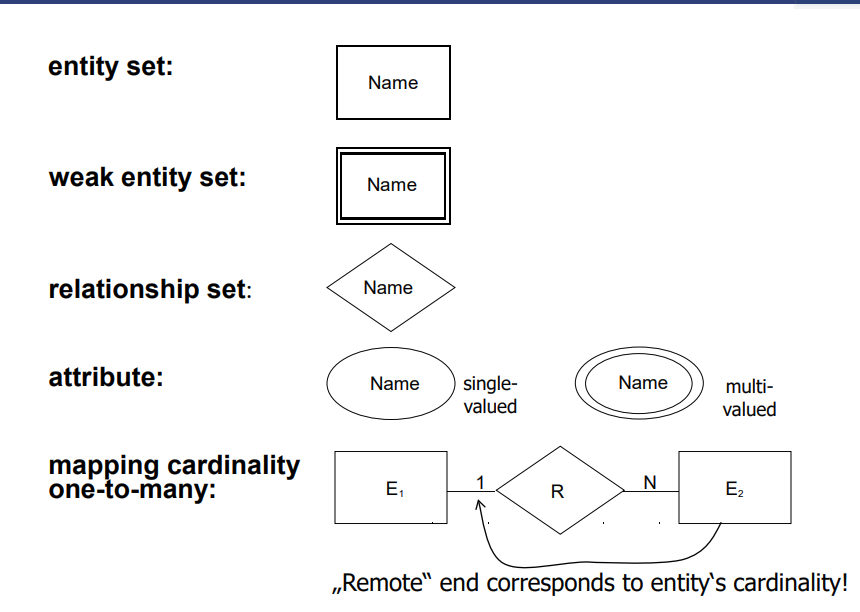
\includegraphics[scale=0.6]{assets/entity_relationship_diagram.png}
\end{document}



